% This LaTeX was auto-generated from MATLAB code.
% To make changes, update the MATLAB code and export to LaTeX again.

\documentclass{article}

\usepackage[utf8]{inputenc}
\usepackage[T1]{fontenc}
\usepackage{lmodern}
\usepackage{graphicx}
\usepackage{color}
\usepackage{hyperref}
\usepackage{amsmath}
\usepackage{amsfonts}
\usepackage{epstopdf}
\usepackage[table]{xcolor}
\usepackage{matlab}

\sloppy
\epstopdfsetup{outdir=./}
\graphicspath{ {./labeling_with_COCO_stuff_resnet_images/} }

\matlabhastoc

\matlabmultipletitles

\begin{document}

\label{H_CDFC31FF}
\matlabheading{License}

\begin{par}
\begin{flushleft}
Please cite the following publication when using or adapting this software or substantial portion thereof for work resulting a publication:
\end{flushleft}
\end{par}

\begin{par}
\begin{flushleft}
Rose O., Johnson J.K., Wang B. and Ponce C.R.; Visual prototypes in the ventral stream are attuned to complexity and gaze behaviour; Nat. Commun; 2021
\end{flushleft}
\end{par}

\begin{par}
\begin{flushleft}
(also see the CITATION file)
\end{flushleft}
\end{par}


\vspace{1em}
\begin{par}
\begin{flushleft}
MIT License
\end{flushleft}
\end{par}

\begin{par}
\begin{flushleft}
Copyright (c) 2021 PonceLab
\end{flushleft}
\end{par}

\begin{par}
\begin{flushleft}
Permission is hereby granted, free of charge, to any person obtaining a copy of this software and associated documentation files (the "Software"), to deal in the Software without restriction, including without limitation the rights to use, copy, modify, merge, publish, distribute, sublicense, and/or sell copies of the Software, and to permit persons to whom the Software is furnished to do so, subject to the following conditions:
\end{flushleft}
\end{par}

\begin{par}
\begin{flushleft}
The above copyright notice and this permission notice shall be included in all copies or substantial portions of the Software.
\end{flushleft}
\end{par}

\begin{par}
\begin{flushleft}
THE SOFTWARE IS PROVIDED "AS IS", WITHOUT WARRANTY OF ANY KIND, EXPRESS OR IMPLIED, INCLUDING BUT NOT LIMITED TO THE WARRANTIES OF MERCHANTABILITY, FITNESS FOR A PARTICULAR PURPOSE AND NONINFRINGEMENT. IN NO EVENT SHALL THE AUTHORS OR COPYRIGHT HOLDERS BE LIABLE FOR ANY CLAIM, DAMAGES OR OTHER LIABILITY, WHETHER IN AN ACTION OF CONTRACT, TORT OR OTHERWISE, ARISING FROM, OUT OF OR IN CONNECTION WITH THE SOFTWARE OR THE USE OR OTHER DEALINGS IN THE SOFTWARE.
\end{flushleft}
\end{par}

\begin{matlabcode}
% add the necessary files to the path (this should be all that is required)
addpath(genpath(pwd))
addpath(genpath(fullfile(fileparts(pwd),'data')))
addpath(genpath(fullfile(fileparts(pwd),'utils')))
\end{matlabcode}

\label{T_670EB89A}
\matlabtitle{Analyzing image content with fuzzy-semantic segmentation}

\matlabtableofcontents{Table of Contents}
\label{T_5C7E8D17}
\begin{par}
\begin{flushleft}
This livescript demonstrates a way to use image labeling to quantitatively score the semantic content of image sets relative to one another. This is in contrast to other image labeling methods which are more precise, but the cost of precision is that quantitative comparison is difficult. 
\end{flushleft}
\end{par}

\label{T_C7724501}
\matlabtitle{Prerequisites, do not ignore!}

\begin{par}
\begin{flushleft}
We have included a fork of \href{https://github.com/kazuto1011/deeplab-pytorch}{deeplab-pytorch} within this repo.  It must still be installed and configured to run with MATLAB. 
\end{flushleft}
\end{par}

\begin{par}
\begin{flushleft}
We recommend against using a virtual enviroment because it can be more complex to make it compatible with MATLAB. However it is not impossible to tell MATLAB to use a specific environment, it is just more stable with the base Anaconda environment. Once everything is downloaded and installed the original authors of \href{https://github.com/kazuto1011/deeplab-pytorch}{deeplab-pytorch} recommended using these commands in the Anaconda prompt:
\end{flushleft}
\end{par}

\begin{verbatim}
# Set up with Anaconda
conda env create -f deeplab-pytorch-master/configs/conda_env.yaml
conda activate deeplab-pytorch
\end{verbatim}
\begin{par}
\begin{flushleft}
\underline{We recommend just opening the file: }\texttt{\underline{deeplab-pytorch-master/configs/conda\_env.yaml }}\underline{and manually installing the dependencies. }
\end{flushleft}
\end{par}

\begin{par}
\begin{flushleft}
You will also need to install \texttt{pydensecrf }which can be done from the Anaconda prompt with this command. 
\end{flushleft}
\end{par}

\begin{verbatim}
pip install git+https://github.com/lucasb-eyer/pydensecrf.git
\end{verbatim}
\begin{par}
\begin{flushleft}
You will then need to install the pretrained model weights, but are likely to have trouble using wget. So you may manually download the weights at the URLs indicated in the file \texttt{deeplab-pytorch-master/scripts/setup\_caffemodels.sh} and place them where indicated. 
\end{flushleft}
\end{par}

\begin{par}
\begin{flushleft}
The bash script which downloads the weights can be run like this:
\end{flushleft}
\end{par}

\begin{verbatim}
$ bash deeplab-pytorch-master/scripts/setup_caffemodels.sh
\end{verbatim}
\begin{par}
\begin{flushleft}
After placing the model weights in the right folders you will need to run convert.py on the coco dataset
\end{flushleft}
\end{par}

\begin{verbatim}
python convert.py --dataset coco
\end{verbatim}
\begin{par}
\begin{flushleft}
Only now can you expect MATLAB to run this code, and that is IF you configured MATLAB to work with python correctly. See other tutorial xxx
\end{flushleft}
\end{par}

\label{T_9ABDA97D}
\matlabtitle{Analyzing image content with a resNet image segmentation and labeling network trained on the COCO-stuff data set}

\begin{par}
\begin{flushleft}
This livescript provides functions for conducting an image content analysis by exploiting a neural network designed to segment an image and use plain english to label the segments. The segments are created by using a conditional random field. This algorithm starts with a list of labels for every pixel and an enumeration of the likelihood that each label appropriately describes the image in the vicinity of that pixel. The conditional random field uses the information from each pixel and its neighbors to narrow it down to the singel label which is most likely to be applicable. A segment is defined as a contiguous region of pixels with the same label. The pixelwise map of labels and label likelihoods is computed by a deep neural network with a resNet architecture. The conditional random field and resNet were freely provided in this implemention (\href{https://github.com/kazuto1011/deeplab-pytorch}{link}) of results from this publication (\href{https://arxiv.org/abs/1606.00915}{link}, [1]). The set of labels and ground truth segmentations used to train that architecture was provided as the COCO-stuff dataset (\href{https://github.com/nightrome/cocostuff}{link} [2]). Importantly, we have modified the application of the conditional random field to permit multiple segmentations. Doing this increases the chance that at least one of the labels for each pixel is the ground truth (if one exists). Furthermore it provides redundancy such that if no label is entirely applicable, the set of labels will have the true label as a point of commonality. The COCO-stuff data set provides a hierarchical grouping of labels by increasingly generalized semantic categories. In most cases the set of labels for each pixel will be concentrated in one of the groups at a more generalized level of the hierarchy. Thus the generalized label serves as a point of commonality, and supplants the need for conjecturizing. Thus we have an effective way to score the semantic content of images that is impartial to the proclivities of any human interpreter. 
\end{flushleft}
\end{par}

\begin{par}
\begin{flushleft}
The modification we made to allow for multiple segmentations and thus multiple labels per-image is the following: First conduct a segmention to choose a label for each pixel. Then, for each pixel, the likelihood of the chosen label is reassigned to be the least likely label. The segmentation is conducted again and the process repeated a set number of times. Given the effect of neighbors it is possible (but rare) for some pixels to be assigned the same label twice.
\end{flushleft}
\end{par}


\vspace{1em}
\begin{par}
\begin{flushleft}
1 - Chen, L. C., Papandreou, G., Kokkinos, I., Murphy, K. \& Yuille, A. L. DeepLab: Semantic Image Segmentation with Deep Convolutional Nets, Atrous Convolution, and Fully Connected CRFs. \textit{IEEE Trans. Pattern Anal. Mach. Intell.} \textbf{40}, 834–848 (2018).
\end{flushleft}
\end{par}

\begin{par}
\begin{flushleft}
2 - Caesar, H., Uijlings, J. \& Ferrari, V. COCO-Stuff: Thing and Stuff Classes in Context. in \textit{Proceedings of the IEEE Computer Society Conference on Computer Vision and Pattern Recognition} 1209–1218 (IEEE Computer Society, 2018). doi:10.1109/CVPR.2018.00132
\end{flushleft}
\end{par}


\vspace{1em}

\vspace{1em}
\label{H_4468301E}
\matlabheading{Single image example}

\begin{par}
\begin{flushleft}
First we will provide an example of running the segmentation and labeling on a single image. This will help you to understand the steps fo the process and how data is structured. 
\end{flushleft}
\end{par}


\vspace{1em}
\label{H_F161908E}
\matlabheadingthree{Output the segmentation maps}

\begin{par}
\hfill \break
\end{par}

\begin{matlabcode}
 % There is a test image already located in the fork of deeplab-pytorch
 % you need only to provide a path to the image, see the help for what parameters are available. These are as used in Rose et al. 
 imagePath=".\image.jpg"
\end{matlabcode}
\begin{matlaboutput}
imagePath = ".\image.jpg"
\end{matlaboutput}
\begin{matlabcode}
[maps,resNetParams]=getLabelMaps(imagePath)
\end{matlabcode}
\begin{matlaboutput}
Device: CPU
Model: DeepLabV2_ResNet101_MSC
maps = 
    labelMapList: [513x513x10 double]
     probMapList: [513x513x10x182 double]
       classList: [1x1 py.dict]

resNetParams = 
      configPath: ".\configs\cocostuff164k.yaml"
       modelPath: ".\data\models\coco\deeplabv1_resnet101\caffemodel\deeplabv2_resnet101_msc-cocostuff164k-100000.pth"
       imagePath: ".\image.jpg"
            cuda: 0
             crf: 1
      sizeThresh: 0.1111
    maxIteration: 10

\end{matlaboutput}

\begin{par}
\begin{flushleft}
\texttt{maps.labelMapList} has 10 slices on the third dimension. Each slice is one iteration from our modifications to the segmentation and labeling process. The original process assigned one label to each pixel. Here we simply repeat that process, but for each iteration we eliminate the most widely assigned labels. Thus, for most pixels the labeling process is forced to pick a different label at each iteration. 
\end{flushleft}
\end{par}

\begin{par}
\begin{flushleft}
\texttt{maps.probMapList} has 182 slices on the forth dimension in addition to the 10 slices on the third. The resNet actually assigns a probability distribution over labels and there are 182 labels for the COCO-stuff data set. In order to pick just one label for each pixel the original model used a "conditional random field" to assess what label had the highest probability for each pixel and take into account the neighbors of that pixel. So all we really did was to force more and more labels to have the lowest probability with each iteration. 
\end{flushleft}
\end{par}


\vspace{1em}
\label{H_050E1979}
\matlabheadingthree{Output the widely applied labels}

\begin{par}
\hfill \break
\end{par}

\begin{matlabcode}
% just provide the outputs of the previous functions
[cloud]=convertMaps2Wordcloud(maps,resNetParams)
\end{matlabcode}
\begin{matlaboutput}
cloud = 
             nLayers: 10
           segImSize: [513 513]
        sortedLabels: [25x1 double]
    sortedClassNames: {25x1 cell}
          labelLayer: [25x1 double]
             nLabels: 25

\end{matlaboutput}

\begin{par}
\begin{flushleft}
\texttt{cloud.sortedClassNames} is a list indicating which of the 182 COC-stuff labels were widely assigned throughout the assignment iterations. It is in order from first iteration (most confident) to last generation (least confident). 
\end{flushleft}
\end{par}

\begin{par}
\begin{flushleft}
\texttt{cloud.sortedLabels} is the same as \texttt{cloud.sortedClassNames}, except is a numerical index into the set of 182. 
\end{flushleft}
\end{par}

\begin{par}
\begin{flushleft}
\texttt{cloud.labelLayer} specifically identifies the iteration (AKA the "layer") in which the assignment was made. 
\end{flushleft}
\end{par}

\begin{par}
\begin{flushleft}
\texttt{cloud.segImSize} is the size of the image that was segmented.
\end{flushleft}
\end{par}


\vspace{1em}
\label{H_1A241096}
\matlabheadingthree{Output relationships between layers}

\begin{par}
\begin{flushleft}
It helps to get a sense of how the algorithm thinks labels are related in an image. This function gives you several adjacency matrices showing pairwise relationships between all identified labels. It also provides the centroids of the labels. This is used for plotting. 
\end{flushleft}
\end{par}

\begin{matlabcode}
[adjMat]=getLabelRelationships(cloud,maps)
\end{matlabcode}
\begin{matlaboutput}
adjMat = 
       labelNetworkOverlap: [25x25 double]
    labelNetworkOverlapDir: [25x25 double]
     labelNetworkJointProb: [25x25 double]
        labelNetworkRelEnt: [25x25 double]
               labelLocMap: [513x513 double]
               labelClusts: [25x1 double]
            labelCentroids: [25x2 double]

\end{matlaboutput}

\begin{par}
\begin{flushleft}
\texttt{adjMat.labelNetworkOverlap} indicates the ratio of the number of pixels that occur in both of two labels relative to the total number of pixels in those labels.
\end{flushleft}
\end{par}

\begin{par}
\begin{flushleft}
\texttt{adjMat.labelNetworkOverlapDir} indicates the ratio of the number of pixels that occur in both of two labels relative to the number of pixels in only one of those labels (the label on the row).
\end{flushleft}
\end{par}

\begin{par}
\begin{flushleft}
\texttt{adjMat.labelNetworkJointProb} indicates the product of all pixelwise probabilities of the labels on the row and column. 
\end{flushleft}
\end{par}

\begin{par}
\begin{flushleft}
\texttt{adjMat.labelNetworkRelEnt} indicates the relative entropy between two labels relative to the label on the row.
\end{flushleft}
\end{par}

\begin{par}
\begin{flushleft}
\texttt{adjMat.labelLocMap} applies the first assigned label to each pixel in the original image.
\end{flushleft}
\end{par}

\begin{par}
\begin{flushleft}
\texttt{adjMat.labelClusts} identifies a hierarchical clustering of labels, to identify which labels have a lot in common.
\end{flushleft}
\end{par}

\begin{par}
\begin{flushleft}
\texttt{adjMat.labelCentroids} is the column, and row of the centroid of the labels in \texttt{adjMat.labelLocMap} 
\end{flushleft}
\end{par}



\vspace{1em}
\label{H_D30FBB80}
\matlabheadingthree{Visualize the label relationships and the labels in the image}

\begin{par}
\hfill \break
\end{par}

\begin{matlabcode}
imagePath=fullfile('.\deeplab-pytorch-master',resNetParams.imagePath);
visualizeSingleSemanticLabelCloud(imagePath,cloud.labelLayer,cloud.sortedClassNames,adjMat.labelLocMap,adjMat.labelNetworkOverlap);
\end{matlabcode}
\begin{center}
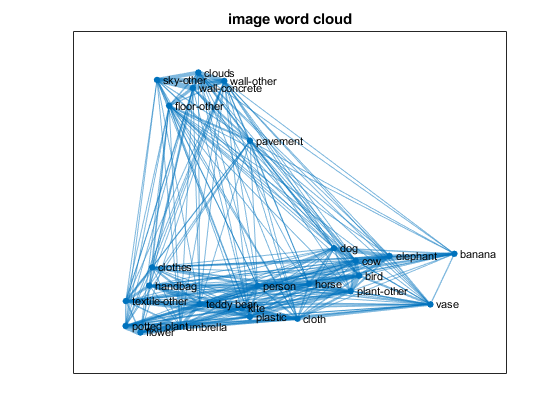
\includegraphics[width=\maxwidth{56.196688409433015em}]{figure_0.png}
\end{center}
\begin{center}
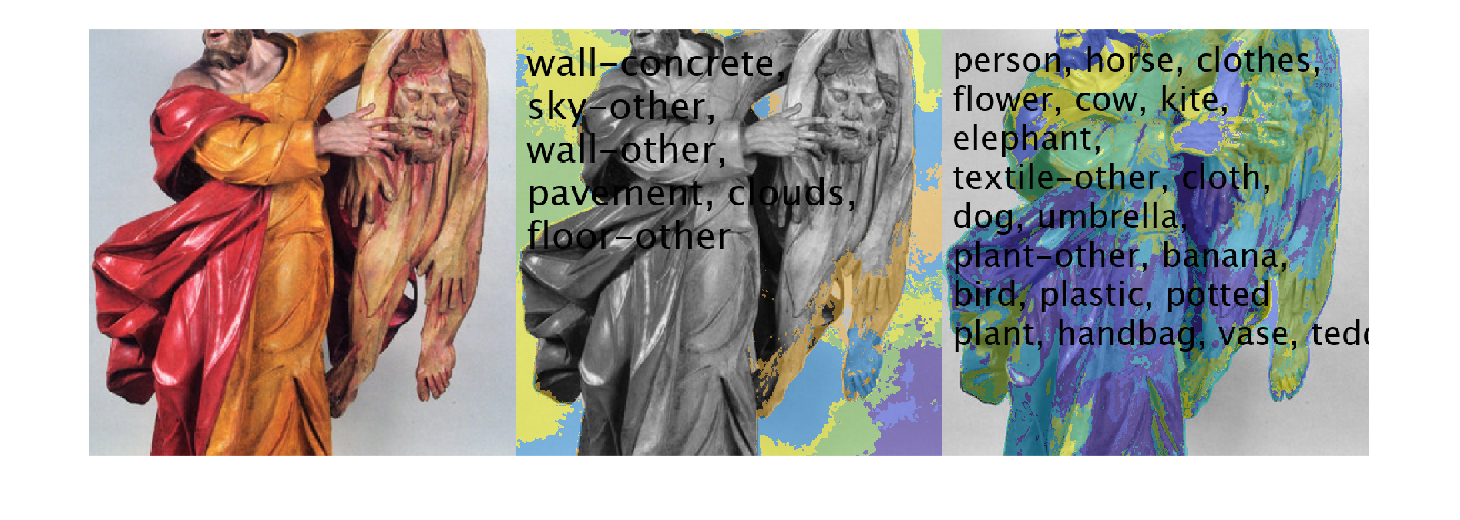
\includegraphics[width=\maxwidth{146.5127947817361em}]{figure_1.png}
\end{center}


\vspace{1em}


\vspace{1em}
\label{H_4FEF4388}
\matlabheading{Example with set of images}

\begin{par}
\begin{flushleft}
Having obtained a set of labels for a single image we now demonstrate counting label occurance frequencies in two sets of images. 
\end{flushleft}
\end{par}

\begin{matlabcode}
% two small samples from AlexNet
daisies=dir('..\data\daisy\*.JPEG');
macaques=dir('..\data\macaque\*.JPEG');
imPaths={fullfile({daisies.folder},{daisies.name}),fullfile({macaques.folder},{macaques.name})};


[classNames,hierarchyLabels]=getClassesYHierarchy();
data2Analyze=cell(size(imPaths));

% get labels and count them without regard to hierarchy
% Note: In our experience, to run this loop in parallel you need separate MATLAB sessions or else you run into stability issues (hangs) due to python integration.
labelCounts=zeros(length(imPaths),length(classNames));
for imType=1:length(imPaths)
    data2Analyze{imType}=cell(1,length(imPaths{imType}));
    for imNdx=1:length(imPaths{imType})
        [maps,resNetParams]=getLabelMaps(imPaths{imType}{imNdx});
        [data2Analyze{imType}{imNdx}]=convertMaps2Wordcloud(maps,resNetParams);
        labelCounts(imType,data2Analyze{imType}{imNdx}.sortedLabels+1)=labelCounts(imType,data2Analyze{imType}{imNdx}.sortedLabels+1)+1;
    end
end
\end{matlabcode}
\begin{matlaboutput}
Device: CPU
Model: DeepLabV2_ResNet101_MSC
Device: CPU
Model: DeepLabV2_ResNet101_MSC
Device: CPU
Model: DeepLabV2_ResNet101_MSC
Device: CPU
Model: DeepLabV2_ResNet101_MSC
Device: CPU
Model: DeepLabV2_ResNet101_MSC
Device: CPU
Model: DeepLabV2_ResNet101_MSC
Device: CPU
Model: DeepLabV2_ResNet101_MSC
Device: CPU
Model: DeepLabV2_ResNet101_MSC
Device: CPU
Model: DeepLabV2_ResNet101_MSC
Device: CPU
Model: DeepLabV2_ResNet101_MSC
Device: CPU
Model: DeepLabV2_ResNet101_MSC
Device: CPU
Model: DeepLabV2_ResNet101_MSC
Device: CPU
Model: DeepLabV2_ResNet101_MSC
Device: CPU
Model: DeepLabV2_ResNet101_MSC
Device: CPU
Model: DeepLabV2_ResNet101_MSC
Device: CPU
Model: DeepLabV2_ResNet101_MSC
Device: CPU
Model: DeepLabV2_ResNet101_MSC
Device: CPU
Model: DeepLabV2_ResNet101_MSC
Device: CPU
Model: DeepLabV2_ResNet101_MSC
Device: CPU
Model: DeepLabV2_ResNet101_MSC
\end{matlaboutput}
\begin{matlabcode}
labelFreqs=labelCounts./sum(labelCounts,2);

% print all the labels and their frequencies for each category
daisyReport=cellfun(@(x) [classNames{x},' = ',num2str(labelCounts(1,x)),';     '],num2cell(1:length(classNames)),'Uni',false);
macaqueReport=cellfun(@(x) [classNames{x},' = ',num2str(labelCounts(1,x)),';     '],num2cell(1:length(classNames)),'Uni',false);

disp(['Daisy, all label counts: ',newline,strjoin(daisyReport,''),newline,newline,newline,newline,'Macaque, all label counts: ',newline,strjoin(macaqueReport,''),newline])
\end{matlabcode}
\begin{matlaboutput}
Daisy, all label counts: 
person = 6;     bicycle = 0;     car = 0;     motorcycle = 0;     airplane = 0;     bus = 0;     train = 0;     truck = 0;     boat = 0;     traffic light = 0;     fire hydrant = 0;     street sign = 0;     stop sign = 0;     parking meter = 0;     bench = 4;     bird = 9;     cat = 3;     dog = 1;     horse = 0;     sheep = 0;     cow = 0;     elephant = 0;     bear = 0;     zebra = 0;     giraffe = 0;     hat = 0;     backpack = 0;     umbrella = 7;     shoe = 0;     eye glasses = 0;     handbag = 0;     tie = 0;     suitcase = 0;     frisbee = 0;     skis = 0;     snowboard = 0;     sports ball = 0;     kite = 0;     baseball bat = 0;     baseball glove = 0;     skateboard = 0;     surfboard = 0;     tennis racket = 0;     bottle = 0;     plate = 0;     wine glass = 0;     cup = 0;     fork = 0;     knife = 0;     spoon = 0;     bowl = 4;     banana = 4;     apple = 1;     sandwich = 0;     orange = 0;     broccoli = 3;     carrot = 0;     hot dog = 0;     pizza = 0;     donut = 0;     cake = 1;     chair = 6;     couch = 1;     potted plant = 10;     bed = 1;     mirror = 0;     dining table = 5;     window = 0;     desk = 0;     toilet = 0;     door = 0;     tv = 0;     laptop = 0;     mouse = 0;     remote = 0;     keyboard = 0;     cell phone = 0;     microwave = 0;     oven = 0;     toaster = 0;     sink = 0;     refrigerator = 0;     blender = 0;     book = 0;     clock = 0;     vase = 10;     scissors = 0;     teddy bear = 0;     hair drier = 0;     toothbrush = 1;     hair brush = 0;     banner = 0;     blanket = 1;     branch = 8;     bridge = 0;     building-other = 3;     bush = 8;     cabinet = 0;     cage = 1;     cardboard = 0;     carpet = 0;     ceiling-other = 2;     ceiling-tile = 0;     cloth = 1;     clothes = 0;     clouds = 0;     counter = 0;     cupboard = 0;     curtain = 1;     desk-stuff = 0;     dirt = 4;     door-stuff = 0;     fence = 7;     floor-marble = 0;     floor-other = 2;     floor-stone = 0;     floor-tile = 1;     floor-wood = 0;     flower = 10;     fog = 0;     food-other = 2;     fruit = 4;     furniture-other = 6;     grass = 8;     gravel = 0;     ground-other = 9;     hill = 3;     house = 1;     leaves = 10;     light = 1;     mat = 0;     metal = 0;     mirror-stuff = 1;     moss = 5;     mountain = 0;     mud = 0;     napkin = 0;     net = 0;     paper = 0;     pavement = 0;     pillow = 0;     plant-other = 10;     plastic = 0;     platform = 0;     playingfield = 0;     railing = 0;     railroad = 0;     river = 0;     road = 0;     rock = 0;     roof = 0;     rug = 0;     salad = 1;     sand = 0;     sea = 0;     shelf = 1;     sky-other = 4;     skyscraper = 0;     snow = 0;     solid-other = 4;     stairs = 0;     stone = 0;     straw = 5;     structural-other = 0;     table = 5;     tent = 0;     textile-other = 4;     towel = 0;     tree = 8;     vegetable = 4;     wall-brick = 1;     wall-concrete = 5;     wall-other = 10;     wall-panel = 2;     wall-stone = 1;     wall-tile = 0;     wall-wood = 5;     water-other = 1;     waterdrops = 0;     window-blind = 0;     window-other = 10;     wood = 7;     



Macaque, all label counts: 
person = 6;     bicycle = 0;     car = 0;     motorcycle = 0;     airplane = 0;     bus = 0;     train = 0;     truck = 0;     boat = 0;     traffic light = 0;     fire hydrant = 0;     street sign = 0;     stop sign = 0;     parking meter = 0;     bench = 4;     bird = 9;     cat = 3;     dog = 1;     horse = 0;     sheep = 0;     cow = 0;     elephant = 0;     bear = 0;     zebra = 0;     giraffe = 0;     hat = 0;     backpack = 0;     umbrella = 7;     shoe = 0;     eye glasses = 0;     handbag = 0;     tie = 0;     suitcase = 0;     frisbee = 0;     skis = 0;     snowboard = 0;     sports ball = 0;     kite = 0;     baseball bat = 0;     baseball glove = 0;     skateboard = 0;     surfboard = 0;     tennis racket = 0;     bottle = 0;     plate = 0;     wine glass = 0;     cup = 0;     fork = 0;     knife = 0;     spoon = 0;     bowl = 4;     banana = 4;     apple = 1;     sandwich = 0;     orange = 0;     broccoli = 3;     carrot = 0;     hot dog = 0;     pizza = 0;     donut = 0;     cake = 1;     chair = 6;     couch = 1;     potted plant = 10;     bed = 1;     mirror = 0;     dining table = 5;     window = 0;     desk = 0;     toilet = 0;     door = 0;     tv = 0;     laptop = 0;     mouse = 0;     remote = 0;     keyboard = 0;     cell phone = 0;     microwave = 0;     oven = 0;     toaster = 0;     sink = 0;     refrigerator = 0;     blender = 0;     book = 0;     clock = 0;     vase = 10;     scissors = 0;     teddy bear = 0;     hair drier = 0;     toothbrush = 1;     hair brush = 0;     banner = 0;     blanket = 1;     branch = 8;     bridge = 0;     building-other = 3;     bush = 8;     cabinet = 0;     cage = 1;     cardboard = 0;     carpet = 0;     ceiling-other = 2;     ceiling-tile = 0;     cloth = 1;     clothes = 0;     clouds = 0;     counter = 0;     cupboard = 0;     curtain = 1;     desk-stuff = 0;     dirt = 4;     door-stuff = 0;     fence = 7;     floor-marble = 0;     floor-other = 2;     floor-stone = 0;     floor-tile = 1;     floor-wood = 0;     flower = 10;     fog = 0;     food-other = 2;     fruit = 4;     furniture-other = 6;     grass = 8;     gravel = 0;     ground-other = 9;     hill = 3;     house = 1;     leaves = 10;     light = 1;     mat = 0;     metal = 0;     mirror-stuff = 1;     moss = 5;     mountain = 0;     mud = 0;     napkin = 0;     net = 0;     paper = 0;     pavement = 0;     pillow = 0;     plant-other = 10;     plastic = 0;     platform = 0;     playingfield = 0;     railing = 0;     railroad = 0;     river = 0;     road = 0;     rock = 0;     roof = 0;     rug = 0;     salad = 1;     sand = 0;     sea = 0;     shelf = 1;     sky-other = 4;     skyscraper = 0;     snow = 0;     solid-other = 4;     stairs = 0;     stone = 0;     straw = 5;     structural-other = 0;     table = 5;     tent = 0;     textile-other = 4;     towel = 0;     tree = 8;     vegetable = 4;     wall-brick = 1;     wall-concrete = 5;     wall-other = 10;     wall-panel = 2;     wall-stone = 1;     wall-tile = 0;     wall-wood = 5;     water-other = 1;     waterdrops = 0;     window-blind = 0;     window-other = 10;     wood = 7;     
\end{matlaboutput}

\begin{par}
\begin{flushleft}
In the above we can see that there are a lot of labels and some small differences. It will help to group labels by similarity. Thankfully, the COCO-stuff data set provides a hierarchy for doing so.
\end{flushleft}
\end{par}


\vspace{1em}


\vspace{1em}
\begin{matlabcode}
% now re-group the labels by the 3rd level of the hierarchy
pick3rd=@(x) x(1:3);
pick1st=@(x) strjoin(x([1,3]),' ');
hierarchyLabels2=hierarchyLabels;
hierarchyNdcsOriginal=grp2idx(hierarchyLabels2);
hierarchyLabels2=categorical(cellfun(@(x) strjoin(fliplr(pick3rd(strsplit(x,' '))),' '),hierarchyLabels2,'Uni',false));
categories2Plot=categories(hierarchyLabels2);
hierarchyNdcs=grp2idx(hierarchyLabels2);

hierarchLabelCounts=zeros([length(imPaths),length(categories2Plot)]);
for imType=1:length(imPaths)
        hierarchLabelCounts(imType,:)=accumarray(hierarchyNdcs,labelCounts(imType,:),[length(categories2Plot),1],@sum);
end
hierarchLabelFreqs=hierarchLabelCounts./sum(hierarchLabelCounts,2);


% print all the labels and their frequencies for each category
daisyReport=cellfun(@(x) [categories2Plot{x},' = ',num2str(hierarchLabelCounts(1,x)),';     '],num2cell(1:length(categories2Plot)),'Uni',false);
macaqueReport=cellfun(@(x) [categories2Plot{x},' = ',num2str(hierarchLabelCounts(1,x)),';     '],num2cell(1:length(categories2Plot)),'Uni',false);


labelOccuranceDiffs=-diff(hierarchLabelFreqs,[],1);
categories2Plot2=reordercats(categorical(categories2Plot),categories2Plot);
figMain=figure();
ax=axes(figMain);
b=bar(ax,categories2Plot2,labelOccuranceDiffs);
b(1).FaceColor=[1,1,1];
b(1).LineWidth=1;
title('Patch interpretations for 27 label categories')
% xtickLabels=ax.XTickLabel;
xtickLabels=cellfun(@(x) pick1st(strsplit(x,' ')),categories2Plot,'Uni',false);
ax.XTickLabel=xtickLabels;
ax.YTick=[-0.04,0,0.04];
ax.YLabel.String={'label frequency','difference'};
ax.YLim=[-0.1,0.07];
ax.YLabel.Position=[-1.1070   -0.0161   -1.0000];
\end{matlabcode}
\begin{center}
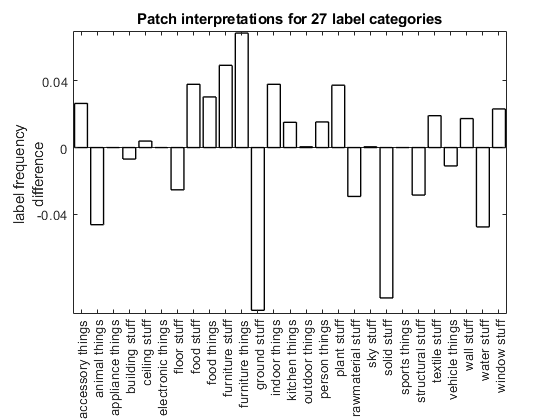
\includegraphics[width=\maxwidth{56.196688409433015em}]{figure_2.png}
\end{center}
\begin{matlabcode}
disp(['Daisy, hierarchy label counts: ',newline,strjoin(daisyReport,''),newline,newline,newline,newline,'Macaque, hierarchy label counts: ',newline,strjoin(macaqueReport,''),newline])
\end{matlabcode}
\begin{matlaboutput}
Daisy, hierarchy label counts: 
accessory outdoor things = 7;     animal outdoor things = 13;     appliance indoor things = 0;     building outdoor stuff = 4;     ceiling indoor stuff = 2;     electronic indoor things = 0;     floor indoor stuff = 3;     food indoor stuff = 11;     food indoor things = 9;     furniture indoor stuff = 14;     furniture indoor things = 23;     ground outdoor stuff = 13;     indoor indoor things = 11;     kitchen indoor things = 4;     outdoor outdoor things = 4;     person outdoor things = 6;     plant outdoor stuff = 72;     rawmaterial indoor stuff = 0;     sky outdoor stuff = 4;     solid outdoor stuff = 14;     sports outdoor things = 0;     structural outdoor stuff = 8;     textile indoor stuff = 7;     vehicle outdoor things = 0;     wall indoor stuff = 24;     water outdoor stuff = 1;     window indoor stuff = 10;     



Macaque, hierarchy label counts: 
accessory outdoor things = 7;     animal outdoor things = 13;     appliance indoor things = 0;     building outdoor stuff = 4;     ceiling indoor stuff = 2;     electronic indoor things = 0;     floor indoor stuff = 3;     food indoor stuff = 11;     food indoor things = 9;     furniture indoor stuff = 14;     furniture indoor things = 23;     ground outdoor stuff = 13;     indoor indoor things = 11;     kitchen indoor things = 4;     outdoor outdoor things = 4;     person outdoor things = 6;     plant outdoor stuff = 72;     rawmaterial indoor stuff = 0;     sky outdoor stuff = 4;     solid outdoor stuff = 14;     sports outdoor things = 0;     structural outdoor stuff = 8;     textile indoor stuff = 7;     vehicle outdoor things = 0;     wall indoor stuff = 24;     water outdoor stuff = 1;     window indoor stuff = 10;     
\end{matlaboutput}

\begin{par}
\begin{flushleft}
While this is easier to interpret there are still many categories and there seems to be a level of noise. It is best to focus only on the labels which rise above the noise. Here we identify those labels and then apply a chi-square test to find differences. 
\end{flushleft}
\end{par}

\begin{matlabcode}

% get only the labels distinguishable from zero
labelFreqSTD=std(hierarchLabelFreqs,[],2);
keepVec=hierarchLabelFreqs>(2*labelFreqSTD); keepVec=any(keepVec,1);
classes2Plot=find(keepVec);
categories2Plot=categories2Plot(classes2Plot);
hierarchLabelFreqsK=hierarchLabelFreqs(:,classes2Plot);
hierarchLabelCountsK=hierarchLabelCounts(:,classes2Plot);

% step through and get the chi square test and odds ratio
nFiles=sum(cellfun(@length,imPaths));
labelStats3rdLevel=cell(length(categories2Plot));
imTypeList=zeros(1,nFiles);
binaryLabelOccurance=zeros(length(classNames),nFiles);
fndx=0;
for imType=1:length(imPaths)
    for imNdx=1:length(imPaths{imType})
fndx=fndx+1;
        imTypeList(fndx)=imType;
        binaryLabelOccurance(data2Analyze{imType}{imNdx}.sortedLabels+1,fndx)=1;
    end
end
    for labelNdx=1:length(categories2Plot)
        labelRemapping=unique(hierarchyNdcsOriginal(hierarchyNdcs==classes2Plot(labelNdx)));
        binaryHierarchLabelOccurance=binaryLabelOccurance(labelRemapping,:); binaryHierarchLabelOccurance=sum(binaryHierarchLabelOccurance,1)~=0;
        [tbl,chi2,p]=crosstab(binaryHierarchLabelOccurance,imTypeList);
        labelStats3rdLevel{labelNdx}={chi2,p,tbl};
    end
labelOccuranceDiffs=-diff(hierarchLabelFreqsK,[],1);

[~,sortedNdcs]=sort(labelOccuranceDiffs,'descend');
categories2Plot=categories2Plot(sortedNdcs);
categories2Plot2=reordercats(categorical(categories2Plot),categories2Plot);
hierarchLabelFreqsK=hierarchLabelFreqsK(sortedNdcs);
hierarchLabelCountsK=hierarchLabelCountsK(sortedNdcs);
labelStats3rdLevel=labelStats3rdLevel(sortedNdcs);
labelOccuranceDiffs=labelOccuranceDiffs(sortedNdcs);



statisticsReport=cellfun(@(x) [categories2Plot{x},': Chi-square = ',num2str(labelStats3rdLevel{x}{1}),', p = ',num2str(labelStats3rdLevel{x}{2}),';     '],num2cell(1:length(categories2Plot)),'Uni',false);


figMain=figure();
ax=axes(figMain);
b=bar(ax,categories2Plot2,labelOccuranceDiffs);
b(1).FaceColor=[1,1,1];
b(1).LineWidth=1;
title('Patch interpretations for the strongest label categories')
% xtickLabels=ax.XTickLabel;
xtickLabels=cellfun(@(x) pick1st(strsplit(x,' ')),categories2Plot,'Uni',false);
sigLevels=cellfun(@(x) (length(categories2Plot)*x{2})<0.05/27,labelStats3rdLevel(:,1));
xtickLabels(sigLevels)=cellfun(@(x) ['*',x],xtickLabels(sigLevels),'Uni',false);
ax.XTickLabel=xtickLabels;
ax.YTick=[-0.04,0,0.04];
ax.YLabel.String={'label frequency','difference'};
ax.YLim=[-0.1,0.041];
ax.YLabel.Position=[-1.1070   -0.0161   -1.0000];
\end{matlabcode}
\begin{center}
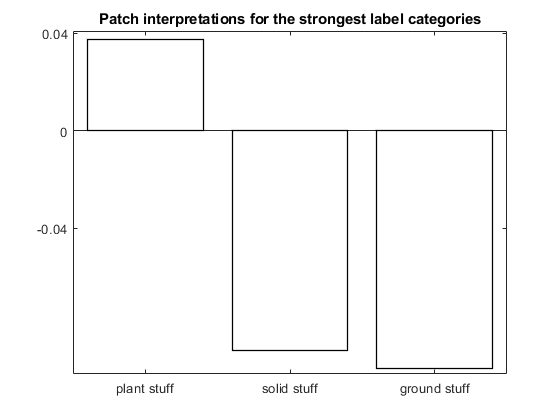
\includegraphics[width=\maxwidth{56.196688409433015em}]{figure_3.png}
\end{center}
\begin{matlabcode}
disp(['Chi-square statistics: ',newline,strjoin(statisticsReport,''),newline])
\end{matlabcode}
\begin{matlaboutput}
Chi-square statistics: 
plant outdoor stuff: Chi-square = NaN, p = NaN;     solid outdoor stuff: Chi-square = 3.5294, p = 0.060289;     ground outdoor stuff: Chi-square = 1.0526, p = 0.3049;     
\end{matlaboutput}

\begin{par}
\begin{flushleft}
The bar chart shows the relative enrichment of one label in the daisy category over the macaque category if values are positive. The reverse is true for negative values. We have also printed the exact chi-square values that correspond to the bon-ferroni significance indicated with * in the plot labels.
\end{flushleft}
\end{par}


\label{T_0DA5B7D5}
\vspace{1em}

\label{T_F4D13F0B}
\matlabtitle{Functions}

\begin{par}
\begin{flushleft}
These are the functions that do all the hardwork. Inspect them to gain a deeper understanding. Copy them for your own use, so long as you cite us!
\end{flushleft}
\end{par}

\begin{matlabcode}
function [maps,resNetParams]=getLabelMaps(imagePath,resNetParams)
% Please cite the following publication when using or adapting this software or substantial portion thereof for work resulting a publication:
% Rose O., Johnson J.K., Wang B. and Ponce C.R.; Visual prototypes in the ventral stream are attuned to complexity and gaze behaviour; Nat. Commun; 2021

if nargin<2 || ~isstruct(resNetParams)
configPath=".\configs\cocostuff164k.yaml";
modelPath=".\data\models\coco\deeplabv1_resnet101\caffemodel\deeplabv2_resnet101_msc-cocostuff164k-100000.pth";

resNetParams=struct('configPath',configPath,'modelPath',modelPath,'imagePath',imagePath,'cuda',false,'crf',true,'sizeThresh',1/9,'maxIteration',10);
end
doPlot=false;

try
    originalDir=pwd;
    cd(".\deeplab-pytorch-master")
catch
    cd("..")
    cd("..")
    originalDir=pwd;
    cd(".\deeplab-pytorch-master")
end
[a]=py.singleHierarchy.singleHierarchy(resNetParams.configPath,resNetParams.modelPath,imagePath,resNetParams.cuda,resNetParams.crf,resNetParams.sizeThresh,resNetParams.maxIteration,doPlot);
imagePath='';
cd(originalDir)

a=cell(a);
maps.labelMapList=cellfun(@(x) double(x), cell(a{1}),'Uni',false); maps.labelMapList=cat(3,maps.labelMapList{:});
maps.probMapList=cellfun(@(x) double(x), cell(a{2}),'Uni',false);  maps.probMapList=permute(cat(4,maps.probMapList{:}),[2,3,4,1]);
maps.classList=a{3};

end


    
function [cloud]=convertMaps2Wordcloud(maps,resNetParams)
% Please cite the following publication when using or adapting this software or substantial portion thereof for work resulting a publication:
% Rose O., Johnson J.K., Wang B. and Ponce C.R.; Visual prototypes in the ventral stream are attuned to complexity and gaze behaviour; Nat. Commun; 2021

    % get a list of all the labels represeneted
    unqLabels=unique(maps.labelMapList(:));
    unqClassNames=cellfun( @(x) char(maps.classList{x}),num2cell(unqLabels),'Uni',false);
    maps.classList=[];
    labelEdges=(unqLabels(1:end-1)+unqLabels(2:end))/2; labelEdges=[unqLabels(1);labelEdges;unqLabels(end)];
    % step through the label maps
    cloud.nLayers=size(maps.labelMapList,3);
    cloud.segImSize=size(maps.labelMapList,[1,2]);
    cloud.sortedLabels=[];
    cloud.sortedClassNames={};
    cloud.labelLayer=[];
    unWrap=@(x) x(:);
    for layer=1:cloud.nLayers
        % keep the unique values which cover more than 1/9th of the image
        N=histcounts(unWrap(maps.labelMapList(:,:,layer)),labelEdges,'Normalization','probability');
        bigLabels=unqLabels(N>=resNetParams.sizeThresh);
        bigClassNames=unqClassNames(N>=resNetParams.sizeThresh);
        % sort them by size and keep track of what level they are in
        % append them to the previous level
        [~,sortNdcs]=sort(N(N>=resNetParams.sizeThresh),'descend');
        cloud.labelLayer=[cloud.labelLayer;layer*ones(size(bigLabels))];
        cloud.sortedLabels=[cloud.sortedLabels;bigLabels(sortNdcs)];
        cloud.sortedClassNames=[cloud.sortedClassNames;bigClassNames(sortNdcs)];
    end
    cloud.nLabels=numel(cloud.sortedLabels);
end


function [adjMat]=getLabelRelationships(cloud,maps)
    % Please cite the following publication when using or adapting this software or substantial portion thereof for work resulting a publication:
% Rose O., Johnson J.K., Wang B. and Ponce C.R.; Visual prototypes in the ventral stream are attuned to complexity and gaze behaviour; Nat. Commun; 2021
    
    % make a blank adjacency matrix
    adjMat.labelNetworkOverlap=zeros(cloud.nLabels);
    adjMat.labelNetworkOverlapDir=zeros(cloud.nLabels);
    adjMat.labelNetworkJointProb=zeros(cloud.nLabels);
    adjMat.labelNetworkRelEnt=zeros(cloud.nLabels);
    % make a deep boolean matrix representing the locations of all the labels represented (in order of the list)
    labelLocs=false([size(maps.labelMapList,[1,2]),numel(cloud.sortedLabels)]);
    probMap=squeeze(maps.probMapList(:,:,1,:)); probMap=probMap./sum(probMap,[1,2]);
    adjMat.labelLocMap=zeros(size(maps.labelMapList,[1,2])); % the sums in this map are uniquely defined by a combination of other layers
    sumLabelCodes=ones(1,cloud.nLabels);
    for labelNdx=1:cloud.nLabels
        label=cloud.sortedLabels(labelNdx);
        labelLocs(:,:,labelNdx)=any(maps.labelMapList==label,3);
        adjMat.labelLocMap(labelLocs(:,:,labelNdx))=adjMat.labelLocMap(labelLocs(:,:,labelNdx))+sumLabelCodes(labelNdx);
        if labelNdx<cloud.nLabels
            sumLabelCodes(labelNdx+1)=sum(sumLabelCodes(1:labelNdx))+1;
        end
    end
    % step through the labels and make the strength of the connection equal to the overlap of sections
    % we could also use joint distribution metrics (KL-divergence, mutual information, etc)
    for rowNdx=1:cloud.nLabels
        for colNdx=1:cloud.nLabels
            if rowNdx==colNdx; continue; end
            if rowNdx>=colNdx
                adjMat.labelNetworkOverlap(rowNdx,colNdx)=sum(labelLocs(:,:,rowNdx) & labelLocs(:,:,colNdx) ,'all')./sum(labelLocs(:,:,rowNdx) | labelLocs(:,:,colNdx) ,'all');
                adjMat.labelNetworkOverlap(colNdx,rowNdx)=adjMat.labelNetworkOverlap(rowNdx,colNdx);
                adjMat.labelNetworkJointProb(rowNdx,colNdx)=sum(exp(log(probMap(:,:,rowNdx))+log(probMap(:,:,colNdx))),'all'); % prevents some round off errors
                adjMat.labelNetworkJointProb(colNdx,rowNdx)=adjMat.labelNetworkJointProb(rowNdx,colNdx);
            end
            adjMat.labelNetworkOverlapDir(rowNdx,colNdx)=sum(labelLocs(:,:,rowNdx) & labelLocs(:,:,colNdx) ,'all')./sum(labelLocs(:,:,rowNdx),'all');
            adjMat.labelNetworkRelEnt(rowNdx,colNdx)=sum(probMap(:,:,rowNdx).*(log(probMap(:,:,rowNdx))-log(probMap(:,:,colNdx))),'all');
        end
    end
    adjMat.labelNetworkOverlap(logical(eye(size(adjMat.labelNetworkOverlap))))=1;
    
    numClusts=min(2,sum(cloud.labelLayer==1));
    [adjMat.labelClusts]=cluster(linkage(squareform(1-adjMat.labelNetworkOverlap),'average'),'maxclust',numClusts);
    
    % visualize by tying each label to it's segment centroid (avoid collisions)
    % step through the labels and get their probability weighted locations
    [cols,rows]=meshgrid(1:cloud.segImSize(2),1:cloud.segImSize(1));
    adjMat.labelCentroids=zeros(cloud.nLabels,2);
    for labelNdx=1:cloud.nLabels
        label=cloud.sortedLabels(labelNdx);
        probMap=maps.probMapList(:,:,1,label+1);
        probMap=probMap(:)./sum(probMap(:));
        adjMat.labelCentroids(labelNdx,:)=round(sum([rows(:).*probMap,cols(:).*probMap],1));
    end
end



function visualizeSingleSemanticLabelCloud(imagePath,labelLayer,sortedClassNames,labelLocMap,labelNetworkAdj)
% Please cite the following publication when using or adapting this software or substantial portion thereof for work resulting a publication:
% Rose O., Johnson J.K., Wang B. and Ponce C.R.; Visual prototypes in the ventral stream are attuned to complexity and gaze behaviour; Nat. Commun; 2021

nLabels=length(labelLayer);
labelLocs=getLabelLocsFromMap(nLabels,labelLocMap);

unDir=all(labelNetworkAdj==labelNetworkAdj',"all");
if unDir
    graphObj=graph(labelNetworkAdj,sortedClassNames,'omitselfloops');
else
    graphObj=digraph(labelNetworkAdj,sortedClassNames,'omitselfloops');
end
labelNetworkAdj=(~eye(size(labelNetworkAdj))).*(labelNetworkAdj+labelNetworkAdj)/2 + eye(size(labelNetworkAdj))*max(labelNetworkAdj(:));
LWidths = 5*graphObj.Edges.Weight/max(graphObj.Edges.Weight);

figure()
p=plot(graphObj,'LineWidth',LWidths,'Layout','force','WeightEffect','inverse');
title('image word cloud')



figure() % plot the main clusters in the image
numClusts=min(2,sum(labelLayer==1));
[splits]=cluster(linkage(squareform(max(labelNetworkAdj(:))-labelNetworkAdj),'average'),'maxclust',numClusts);
numClusts=numel(unique(splits));
if numClusts==1;
numClusts=min(2,sum(labelLayer==1))+1;
[splits]=cluster(linkage(squareform(max(labelNetworkAdj(:))-labelNetworkAdj),'average'),'maxclust',numClusts);
numClusts=numel(unique(splits));
end

if ~isnumeric(imagePath)
    originalImage=imresize(imread(imagePath),size(labelLocMap,[1,2]));
else
    originalImage=imresize(imagePath,size(labelLocMap,[1,2]));
end
grayVersion=repmat(rgb2gray(originalImage),[1,1,3]);
imSize=size(originalImage);
clustMasks=zeros([size(labelLocMap,[1,2]),numClusts]);
clustClouds=cell(1,numClusts);
clustIms=cell(1,numClusts);
for ndx=1:numClusts
    clustMasks(:,:,ndx)=sum(labelLocs(:,:,splits==ndx),3);
    clustClouds{ndx}=sortedClassNames(splits==ndx);
    heatMapOverlay=labeloverlay(grayVersion,clustMasks(:,:,ndx),'Colormap','parula');
    FontSize=round(40+40/length(clustClouds{ndx}));
    % make sure the text fits in the image
    fontWidth=FontSize/2;
    imWidth=ceil(imSize(2)/fontWidth);
    cloudString=strjoin(clustClouds{ndx},', ');
    if length(cloudString)>=imWidth;
        nParts=ceil(length(cloudString)/imWidth);
        newLineLocs=zeros(1,nParts);
        temp=strfind(cloudString,' ');
        if length(temp)<nParts; temp=[temp,length(cloudString)+1]; end
        for insertCnt=1:nParts
            if insertCnt==1
                newLineLocs(insertCnt)=temp(find(temp<((insertCnt-1)*(imWidth-1)+imWidth) & temp>((insertCnt-1)*(imWidth-1)+1),1,'last'));
            else
                newLineLocs(insertCnt)=temp(find(temp<(newLineLocs(insertCnt-1)+imWidth) & temp>newLineLocs(insertCnt-1),1,'last'));
            end
        end
        cloudString(newLineLocs)=newline;
    end
    clustIms{ndx}=insertText(heatMapOverlay,[0,0],cloudString,'BoxOpacity',0,'TextColor',[1,0.97,0.95],'FontSize',FontSize-2);
end
if numClusts<4
montage([originalImage,clustIms],'Size',[1,numClusts+1])
else
montage([originalImage,clustIms])
end
drawnow

end


function labelLocs2=getLabelLocsFromMap(nLabels,labelLocMap)
% Please cite the following publication when using or adapting this software or substantial portion thereof for work resulting a publication:
% Rose O., Johnson J.K., Wang B. and Ponce C.R.; Visual prototypes in the ventral stream are attuned to complexity and gaze behaviour; Nat. Commun; 2021

sumLabelCodes=ones(1,nLabels);
for labelNdx=1:nLabels
    if labelNdx<nLabels
        sumLabelCodes(labelNdx+1)=sum(sumLabelCodes(1:labelNdx))+1;
    end
end
factorList=cell(nLabels,1);
for labNdx=1:nLabels
    factorList{labNdx}=factor(sumLabelCodes(labNdx));
end


isOdd=mod(labelLocMap,2)==1;
labelLocMap2=labelLocMap;
labelLocMap2(isOdd)=max(1,labelLocMap2(isOdd)-1);
labelLocs2=(labelLocMap2==permute(sumLabelCodes,[1,3,2]));
labelLocs2(:,:,1)=labelLocs2(:,:,1)  |  isOdd ;
uniqueSums=unique(labelLocMap2(:));
uniqueSums=setdiff(uniqueSums,sumLabelCodes);
uniqueSums=sort(uniqueSums,'descend');

nSums=numel(uniqueSums);
sumComps=cell(1,nSums);
foundsums=[];
missingSums=uniqueSums;
for sumNdx=1:nSums
    if ~isempty(sumComps{sumNdx}); continue; end
    sumVal=uniqueSums(sumNdx);
    
    % see if the sum has only one component
    knownComponents=sumLabelCodes(sumLabelCodes==sumVal);
    if isempty(knownComponents)
        possibleComponents=sort(sumLabelCodes(sumLabelCodes>1 & sumLabelCodes<sumVal),'descend');
        if sum(possibleComponents)==sumVal % see if the sum is all possible components
            knownComponents=possibleComponents;
        else
            % test all possible combinations
            compRows=possibleComponents'; % the first combination is just the one possible component so the "component rows" is width==1
            sumTest=sum(compRows,2);
            cnt=0;
            while ~any(sumTest==sumVal)
                cnt=cnt+1;
                % make a matrix of the sum of prior combinations  with another set of possible components
                [rows,cols]=meshgrid(1:size(compRows,1),possibleComponents);
                sumTest=possibleComponents'+sumTest'; % here is the matrix
                indexer=sumTest<=sumVal; % get rid of values larger than the sum
                sumTest=sumTest(indexer);
                compRows=sort([compRows(rows(indexer),:),cols(indexer)],2); % list the expanded set of combinations we just tested
                [compRows,indexer]=unique(compRows,'rows'); % the order of components doesn't matter so keep unique rows
                indexer=indexer(~any(diff(compRows,[],2)==0,2)); % no component can be repeated 2 or more times so get rid of repeats
                sumTest=sumTest(indexer);
                compRows=compRows(~any(diff(compRows,[],2)==0,2),:);
                % we might not have found the combination for the sum we are checking but we might have stumbled across another
                checkSums=sumTest==missingSums';
                if any(checkSums,'all')
                    foundSumNdcs=setdiff(find(any(checkSums,1)),foundsums);
                    foundsums=unique([foundSumNdcs,foundsums]);
                    missingSums(foundsums)=0;
                    % disp(['found ',num2str(length(foundSumNdcs)),' other sums'])
                    for foundSumNdx=foundSumNdcs
                        if ~isempty(sumComps{foundSumNdx}); continue; end
                        sumComps{foundSumNdx}=compRows(sum(compRows,2)==uniqueSums(foundSumNdx),:);
                        if size(sumComps{foundSumNdx},1)~=1; error('the labelLocMap is inconsistent with the number of labels'); end
                    end
                end
            end
            knownComponents=compRows(sum(compRows,2)==sumVal,:);
            if size(knownComponents,1)~=1; error('the labelLocMap is inconsistent with the number of labels'); end
        end
    end
    sumComps{sumNdx}=knownComponents;
end

for sumNdx=1:nSums
    knownComponents=sumComps{sumNdx};
    sumVal=uniqueSums(sumNdx);
    labelLocs2(:,:,ismember(sumLabelCodes,knownComponents))=labelLocs2(:,:,ismember(sumLabelCodes,knownComponents)) | labelLocMap2==sumVal;
end

end






function [classNames,hierarchyLabels]=getClassesYHierarchy()



parentsStuff = { ...
    'stuff', 'stuff'; ...
    ... % End of level 1
    'indoor-super-stuff', 'stuff'; ...
    'outdoor-super-stuff', 'stuff'; ...
    ... % End of level 2
    'rawmaterial-stuff', 'indoor-super-stuff'; ...
    'wall-stuff', 'indoor-super-stuff'; ...
    'ceiling-stuff', 'indoor-super-stuff'; ...
    'floor-stuff', 'indoor-super-stuff'; ...
    'window-stuff', 'indoor-super-stuff'; ...
    'furniture-stuff', 'indoor-super-stuff'; ...
    'textile-stuff', 'indoor-super-stuff'; ...
    'food-stuff', 'indoor-super-stuff'; ...
    'building-stuff', 'outdoor-super-stuff'; ...
    'structural-stuff', 'outdoor-super-stuff'; ...
    'plant-stuff', 'outdoor-super-stuff'; ...
    'sky-stuff', 'outdoor-super-stuff'; ...
    'solid-stuff', 'outdoor-super-stuff'; ...
    'ground-stuff', 'outdoor-super-stuff'; ...
    'water-stuff', 'outdoor-super-stuff'; ...
    ... % End of level 3
    'cardboard', 'rawmaterial-stuff'; ...
    'paper', 'rawmaterial-stuff'; ...
    'plastic', 'rawmaterial-stuff'; ...
    'metal', 'rawmaterial-stuff'; ...
    'wall-tile', 'wall-stuff'; ...
    'wall-panel', 'wall-stuff'; ...
    'wall-wood', 'wall-stuff'; ...
    'wall-brick', 'wall-stuff'; ...
    'wall-stone', 'wall-stuff'; ...
    'wall-concrete', 'wall-stuff'; ...
    'wall-other', 'wall-stuff'; ...
    'ceiling-tile', 'ceiling-stuff'; ...
    'ceiling-other', 'ceiling-stuff'; ...
    'carpet', 'floor-stuff'; ...
    'floor-tile', 'floor-stuff'; ...
    'floor-wood', 'floor-stuff'; ...
    'floor-marble', 'floor-stuff'; ...
    'floor-stone', 'floor-stuff'; ...
    'floor-other', 'floor-stuff'; ...
    'window-blind', 'window-stuff'; ...
    'window-other', 'window-stuff'; ...
    'door-stuff', 'furniture-stuff'; ...
    'desk-stuff', 'furniture-stuff'; ...
    'table', 'furniture-stuff'; ...
    'shelf', 'furniture-stuff'; ...
    'cabinet', 'furniture-stuff'; ...
    'cupboard', 'furniture-stuff'; ...
    'mirror-stuff', 'furniture-stuff'; ...
    'counter', 'furniture-stuff'; ...
    'light', 'furniture-stuff'; ...
    'stairs', 'furniture-stuff'; ...
    'furniture-other', 'furniture-stuff'; ...
    'rug', 'textile-stuff'; ...
    'mat', 'textile-stuff'; ...
    'towel', 'textile-stuff'; ...
    'napkin', 'textile-stuff'; ...
    'clothes', 'textile-stuff'; ...
    'cloth', 'textile-stuff'; ...
    'curtain', 'textile-stuff'; ...
    'blanket', 'textile-stuff'; ...
    'pillow', 'textile-stuff'; ...
    'banner', 'textile-stuff'; ...
    'textile-other', 'textile-stuff'; ...
    'fruit', 'food-stuff'; ...
    'salad', 'food-stuff'; ...
    'vegetable', 'food-stuff'; ...
    'food-other', 'food-stuff'; ...
    ... % End of level 4 left
    'house', 'building-stuff'; ...
    'skyscraper', 'building-stuff'; ...
    'bridge', 'building-stuff'; ...
    'tent', 'building-stuff'; ...
    'roof', 'building-stuff'; ...
    'building-other', 'building-stuff'; ...
    'fence', 'structural-stuff'; ...
    'cage', 'structural-stuff'; ...
    'net', 'structural-stuff'; ...
    'railing', 'structural-stuff'; ...
    'structural-other', 'structural-stuff'; ...
    'grass', 'plant-stuff'; ...
    'tree', 'plant-stuff'; ...
    'bush', 'plant-stuff'; ...
    'leaves', 'plant-stuff'; ...
    'flower', 'plant-stuff'; ...
    'branch', 'plant-stuff'; ...
    'moss', 'plant-stuff'; ...
    'straw', 'plant-stuff'; ...
    'plant-other', 'plant-stuff'; ...
    'clouds', 'sky-stuff'; ...
    'sky-other', 'sky-stuff'; ...
    'wood', 'solid-stuff'; ...
    'rock', 'solid-stuff'; ...
    'stone', 'solid-stuff'; ...
    'mountain', 'solid-stuff'; ...
    'hill', 'solid-stuff'; ...
    'solid-other', 'solid-stuff'; ...
    'sand', 'ground-stuff'; ...
    'snow', 'ground-stuff'; ...
    'dirt', 'ground-stuff'; ...
    'mud', 'ground-stuff'; ...
    'gravel', 'ground-stuff'; ...
    'road', 'ground-stuff'; ...
    'pavement', 'ground-stuff'; ...
    'railroad', 'ground-stuff'; ...
    'platform', 'ground-stuff'; ...
    'playingfield', 'ground-stuff'; ...
    'ground-other', 'ground-stuff'; ...
    'fog', 'water-stuff'; ...
    'river', 'water-stuff'; ...
    'sea', 'water-stuff'; ...
    'waterdrops', 'water-stuff'; ...
    'water-other', 'water-stuff'; ...
    };



parentsThings = { ...
    'things', 'things'; ...
    ... % End of level 1
    'indoor-super-things', 'things'; ...
    'outdoor-super-things', 'things'; ...
    ... % End of level 2
    'person-things', 'outdoor-super-things'; ...
    'vehicle-things', 'outdoor-super-things'; ...
    'outdoor-things', 'outdoor-super-things'; ...
    'animal-things', 'outdoor-super-things'; ...
    'accessory-things', 'outdoor-super-things'; ...
    'sports-things', 'outdoor-super-things'; ...
    'kitchen-things', 'indoor-super-things'; ...
    'food-things', 'indoor-super-things'; ...
    'furniture-things', 'indoor-super-things'; ...
    'electronic-things', 'indoor-super-things'; ...
    'appliance-things', 'indoor-super-things'; ...
    'indoor-things', 'indoor-super-things'; ...
    ... % End of level 3
    'person', 'person-things'; ...
    'bicycle', 'vehicle-things'; ...
    'car', 'vehicle-things'; ...
    'motorcycle', 'vehicle-things'; ...
    'airplane', 'vehicle-things'; ...
    'bus', 'vehicle-things'; ...
    'train', 'vehicle-things'; ...
    'truck', 'vehicle-things'; ...
    'boat', 'vehicle-things'; ...
    'traffic light', 'outdoor-things'; ...
    'fire hydrant', 'outdoor-things'; ...
    'street sign', 'outdoor-things'; ...
    'stop sign', 'outdoor-things'; ...
    'parking meter', 'outdoor-things'; ...
    'bench', 'outdoor-things'; ...
    'bird', 'animal-things'; ...
    'cat', 'animal-things'; ...
    'dog', 'animal-things'; ...
    'horse', 'animal-things'; ...
    'sheep', 'animal-things'; ...
    'cow', 'animal-things'; ...
    'elephant', 'animal-things'; ...
    'bear', 'animal-things'; ...
    'zebra', 'animal-things'; ...
    'giraffe', 'animal-things'; ...
    'hat', 'accessory-things'; ...
    'backpack', 'accessory-things'; ...
    'umbrella', 'accessory-things'; ...
    'shoe', 'accessory-things'; ...
    'eye glasses', 'accessory-things'; ...
    'handbag', 'accessory-things'; ...
    'tie', 'accessory-things'; ...
    'suitcase', 'accessory-things'; ...
    'frisbee', 'sports-things'; ...
    'skis', 'sports-things'; ...
    'snowboard', 'sports-things'; ...
    'sports ball', 'sports-things'; ...
    'kite', 'sports-things'; ...
    'baseball bat', 'sports-things'; ...
    'baseball glove', 'sports-things'; ...
    'skateboard', 'sports-things'; ...
    'surfboard', 'sports-things'; ...
    'tennis racket', 'sports-things'; ...
    'bottle', 'kitchen-things'; ...
    'plate', 'kitchen-things'; ...
    'wine glass', 'kitchen-things'; ...
    'cup', 'kitchen-things'; ...
    'fork', 'kitchen-things'; ...
    'knife', 'kitchen-things'; ...
    'spoon', 'kitchen-things'; ...
    'bowl', 'kitchen-things'; ...
    'banana', 'food-things'; ...
    'apple', 'food-things'; ...
    'sandwich', 'food-things'; ...
    'orange', 'food-things'; ...
    'broccoli', 'food-things'; ...
    'carrot', 'food-things'; ...
    'hot dog', 'food-things'; ...
    'pizza', 'food-things'; ...
    'donut', 'food-things'; ...
    'cake', 'food-things'; ...
    'chair', 'furniture-things'; ...
    'couch', 'furniture-things'; ...
    'potted plant', 'furniture-things'; ...
    'bed', 'furniture-things'; ...
    'mirror', 'furniture-things'; ...
    'dining table', 'furniture-things'; ...
    'window', 'furniture-things'; ...
    'desk', 'furniture-things'; ...
    'toilet', 'furniture-things'; ...
    'door', 'furniture-things'
    'tv', 'electronic-things'; ...
    'laptop', 'electronic-things'; ...
    'mouse', 'electronic-things'; ...
    'remote', 'electronic-things'; ...
    'keyboard', 'electronic-things'; ...
    'cell phone', 'electronic-things'; ...
    'microwave', 'appliance-things'; ...
    'oven', 'appliance-things'; ...
    'toaster', 'appliance-things'; ...
    'sink', 'appliance-things'; ...
    'refrigerator', 'appliance-things'; ...
    'blender', 'appliance-things'; ...
    'book', 'indoor-things'; ...
    'clock', 'indoor-things'; ...
    'vase', 'indoor-things'; ...
    'scissors', 'indoor-things'; ...
    'teddy bear', 'indoor-things'; ...
    'hair drier', 'indoor-things'; ...
    'toothbrush', 'indoor-things'; ...
    'hair brush', 'indoor-things'; ...
    };


classNames={'person', 'bicycle', 'car', 'motorcycle', 'airplane', 'bus', 'train', 'truck', 'boat', 'traffic light', 'fire hydrant', 'street sign',...
    'stop sign', 'parking meter', 'bench', 'bird', 'cat', 'dog', 'horse', 'sheep', 'cow', 'elephant', 'bear', 'zebra', 'giraffe', 'hat', 'backpack',...
    'umbrella', 'shoe', 'eye glasses', 'handbag', 'tie', 'suitcase', 'frisbee', 'skis', 'snowboard', 'sports ball', 'kite', 'baseball bat',...
    'baseball glove', 'skateboard', 'surfboard', 'tennis racket', 'bottle', 'plate', 'wine glass', 'cup', 'fork', 'knife', 'spoon', 'bowl',...
    'banana', 'apple', 'sandwich', 'orange', 'broccoli', 'carrot', 'hot dog', 'pizza', 'donut', 'cake', 'chair', 'couch', 'potted plant', 'bed',...
    'mirror', 'dining table', 'window', 'desk', 'toilet', 'door', 'tv', 'laptop', 'mouse', 'remote', 'keyboard', 'cell phone', 'microwave', 'oven',...
    'toaster', 'sink', 'refrigerator', 'blender', 'book', 'clock', 'vase', 'scissors', 'teddy bear', 'hair drier', 'toothbrush', 'hair brush',...
    'banner', 'blanket', 'branch', 'bridge', 'building-other', 'bush', 'cabinet', 'cage', 'cardboard', 'carpet', 'ceiling-other', 'ceiling-tile',...
    'cloth', 'clothes', 'clouds', 'counter', 'cupboard', 'curtain', 'desk-stuff', 'dirt', 'door-stuff', 'fence', 'floor-marble', 'floor-other',...
    'floor-stone', 'floor-tile', 'floor-wood', 'flower', 'fog', 'food-other', 'fruit', 'furniture-other', 'grass', 'gravel', 'ground-other', 'hill',...
    'house', 'leaves', 'light', 'mat', 'metal', 'mirror-stuff', 'moss', 'mountain', 'mud', 'napkin', 'net', 'paper', 'pavement', 'pillow',...
    'plant-other', 'plastic', 'platform', 'playingfield', 'railing', 'railroad', 'river', 'road', 'rock', 'roof', 'rug', 'salad', 'sand', 'sea',...
    'shelf', 'sky-other', 'skyscraper', 'snow', 'solid-other', 'stairs', 'stone', 'straw', 'structural-other', 'table', 'tent', 'textile-other',...
    'towel', 'tree', 'vegetable', 'wall-brick', 'wall-concrete', 'wall-other', 'wall-panel', 'wall-stone', 'wall-tile', 'wall-wood', 'water-other',...
    'waterdrops', 'window-blind', 'window-other', 'wood'};

parents=[parentsStuff;parentsThings];
classParents=cell(length(classNames),3);
for cNdx=1:length(classNames)
    locationsInHierarchy=find(strcmpi(parents(:,1),classNames{cNdx}));
    if length(locationsInHierarchy)~=1
        dsafasdf
    end
    classParents{cNdx,1}=parents{locationsInHierarchy,2};
    locationsInHierarchy=find(strcmpi(parents(:,1),classParents{cNdx,1}));
    if length(locationsInHierarchy)~=1
        dsafasdf2
    end
    classParents{cNdx,2}=parents{locationsInHierarchy,2};
    locationsInHierarchy=find(strcmpi(parents(:,1),classParents{cNdx,2}));
    if length(locationsInHierarchy)~=1
        dsafasdf2
    end
    classParents{cNdx,3}=parents{locationsInHierarchy,2};
end

hierarchyLabels=classNames;
for cNdx=1:length(classNames)
    hierarchyLabels{cNdx}=[classParents{cNdx,3},' ',classParents{cNdx,2}(1:(strfind(classParents{cNdx,2},'-')-1)),' ',classParents{cNdx,1}(1:(strfind(classParents{cNdx,1},'-')-1)),' ',classNames{cNdx}];
end


end













\end{matlabcode}

\end{document}
